% This is samplepaper.tex, a sample chapter demonstrating the
% LLNCS macro package for Springer Computer Science proceedings;
% Version 2.20 of 2017/10/04
%
\documentclass[runningheads]{llncs}
%
\usepackage{graphicx}
\usepackage{dirtytalk}
% Used for displaying a sample figure. If possible, figure files should
% be included in EPS format.
%
% If you use the hyperref package, please uncomment the following line
% to display URLs in blue roman font according to Springer's eBook style:
% \renewcommand\UrlFont{\color{blue}\rmfamily}

\begin{document}
% Welche Aufgaben hat unser System? Was brauchen wir für Komponenten zur Realisierung? Wie können wir die sinnvoll in Threads unterteilen?
\title{Proposal: Chinese Whispers}

\author{Group 1: Nadine Bisswang (804957) \and Johannes Deufel (804958) \and Jonas Pfaff (804930) \and Philipp Straub (804934)}

\institute{}
%
\maketitle              % typeset the header of the contribution
\section{Introduction}
    As part of the Distributed System Project, we would like to implement the game \say{chinese whispers} (german: \say{Stille Post}) in a distributed system as part of the examination performance. 
    This historical children's game primarily serves the perceptual education of children and is didactically very valuable especially at kindergarten age. The goal of the game is for all players involved to correctly pass on a previously selected word or phrase. The attraction of the game (for the kids and educators) results from the fact that the last player has to pronounce what has been passed on aloud - this often results in very funny misunderstandings. 
    
    %In the computer-assisted version, additional points are introduced in order to be able to choose a winner at the end of the game round. Just like in kindergarten, it must also be possible for individual players to leave the circle. Furthermore, the game must continue if the game leaders (educators) have to move away from the group (or, in IT-terms: crash).
    
    It is very exciting to map this game within a distributed system, as it is also formed in reality from many, distributed players. Without the distribution or the participation of at least four players, the game is not playable. Furthermore, the system follows a synchronous approach, since - just like in the real game - you have to wait for the previous player to pass on what he understood.

\section{Project Requirements Analysis}
    \subsection{Dynamic discovery of hosts}
        To enable our solution to be dynamically joined and left, we implement the dynamic discovery of hosts. For a Peer-to-Peer architecture we see different scenarios how dynamic discovery will appear: A peer starts and a network already exists, a peer starts and is the first node of a network or a peer is already a node in a network.
        
        In each of these cases, each peer creates, manages and shares its own group view based on UDP Broadcast and TCP Unicast. This way we can implement a unified group view across the network. Since it is very difficult to play Chinese Whispers alone, each node initially broadcasts its address and listens to the response to find other players. As we consider a ring topology to be the most suitable for this kind of game, we will implement a logic that allows each peer to find its neighbors.
        
    \subsection{Crash fault tolerance}
        To ensure that the game is still working once one of the peers crashes, the system must implement crash fault tolerance. Therefore, each peer receives signals from its two neighbors in the ring topology called heartbeats. Once a heartbeat is missing, the peer can report the absence to rearrange the topology. Additionally, the leader distributes the current game state through an UDP Broadcast after each round. This ensures the continuation of the game if the leader crashes. If the number of peers falls below the minimum number of four, the system waits for new participants to continue.
    
    \subsection{Voting}
        The system must enable initial voting. From this voting a leader emerges, who distributes the points in the game and selects the word from a given list.
        
        In addition, the system must be able to initialize a new voting in case of failure of a peer (if it was the leader) and thus determine a new leader. 
    
        When a new peer joins an existing network, the system also checks whether it becomes the new leader.
    
    \subsection{Reliable multicast} 
        In the system we don't have a central server, which stores the state of the game. Therefore we propose as fourth requirement to implement a reliable multicast. In our system we define one peer who is the leader and establishes the word (which is whispered) at the beginning. This peer passes the first word to it's neighbor (predefined order). This neighbor passes the word to it's neighbor and so on until the last peer in the round, which isn't the leader, receives the word.  
        
        At the end of the game the leader compares the word with the initial word at the beginning. The information about which word came out in the end and whether the word is correct is then distributed to all other peers (reliable multicast). If the leader "dies" our system will vote for a new leader.
    
\section{Architectural Design}
    The de-central organization of the game logic leads to a Peer-to-Peer Network.

    \begin{figure}
        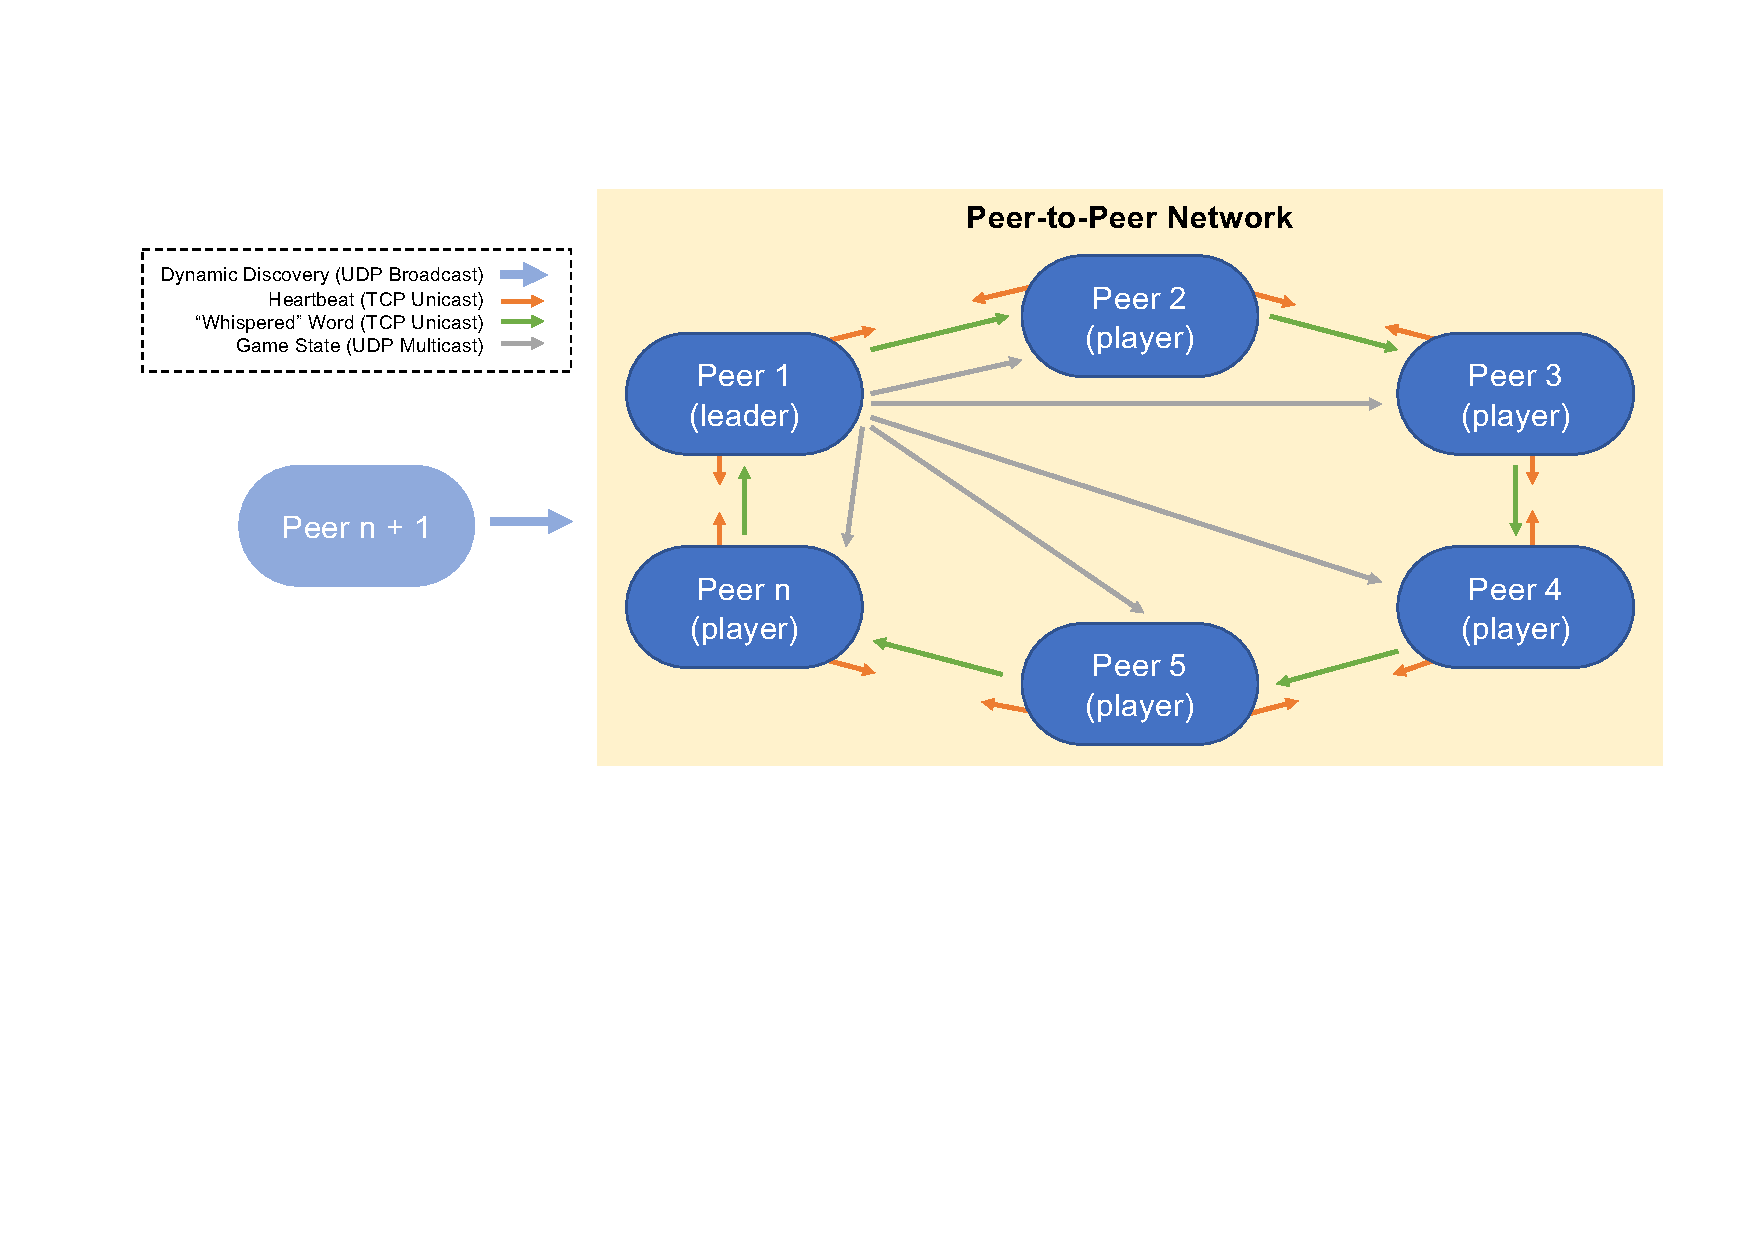
\includegraphics[width=\textwidth]{architecture.pdf}
    \end{figure}

\end{document}